\chapter{Hardware Design and Development of Aerial Robot Swarm Platforms}

One big part of this internship consisted of choosing the hardware of the drone.
Much time was dedicated to researching how to choose the drone's components according to specifications.
Every component had to be the perfect fit for this project.
Different forums, DIY websites, and youtube videos were used as resources to make this guide.
A lot of the criteria are thumb rule, as the domain is mainly hobbyist.
This process is complicated as with the change of one component; other components must be changed to take it into account.
You also have to verify that everything is compatible with the other components.
You have to make sure you also have all the connectors.
And that the autopilot chosen is compatible.
As the components are ordered from China, only one order could be passed during this internship.
There was no place for mistakes.
Some components were ordered in double because of this, as some components are known not always to work.
The components needed to fit on the drone, so the weight and space were significant in the choice.
Also, the components needed to fit together.

\section{Generic Guide to design a drone}

This guide explains how to choose the different components, one by one.

\subsection{Components on the drone}

\subsubsection{Frame}
The choice of the drone frame is critical.
The size of the frame impacts the choice of the propellers, the motors, the ESC, and the battery.
It has to be big enough to have enough space for all the components of the drone.
And, as the aim is to create a swarm of drone, the smaller the drone, the better.

\subsubsection{Props}
The propellers have three significant characteristics: their size, their pitch, and their number of blades.

The size of the propellers, in part fixed by the size of the frame.

The higher the pitch, the higher the thrust, but also, higher torque is needed from the motors.
Moreover, the pitch should always be less than 2/3 of the propeller size as higher pitch could cause air disturbances (Vortex Ring State).
So, the pitch was chosen by taking the highest pitch on the market that respected the 2/3 ratio.

The number of blades impacts thrust and efficiency. More blades mean increased thrust but decreased efficiency.

The propeller specification are generally either \emph{SxPxB} or \emph{SSPPxB}.
S is the size, P the pitch, and B the number of blades
(e.g., for a size of 70mm and pitch of 4.5 and 2 blades, 7x4.5x2 and 7045x2).

\subsubsection{Motors}
The motors have different characteristics. Its width, height, and KV.

These characteristics are, in part, fixed by the frame and the propellers.

Some motors come with a propeller adapter.

\subsubsection{ESCs}
The ESC has to major characteristics, their current limit, and their max voltage input in S unit, number of cells of LiPo battery (e.g., 3S).

The motor current consumption should never exceed the ESC current limit.

It is advised to buy extra spare ESC and oversize them as it is a critical part of the drone.

\subsubsection{Battery}
The battery has a voltage fixed by its number of cells, $3.7V$ nominal per cell.
It has a capacity in mAh,
The current draw the LiPo can support is its capacity times the C-rating.

The motor current consumption should never exceed the maximum current draw of the LiPo.

\subsubsection{Power distribution board}
The PDB has a max current and max voltage that should not be exceeded.

\subsubsection{RC Receiver}
For a drone, the minimum amount of channel for a receiver is 6.
The receiver can either send the received signal via PWM or PPM to the flight controller.

\subsubsection{Flight Controller}
The flight controller is an electronic board with sensors (e.g., accelerometer, gyroscope, barometer).

The choice of a flight controller often depends on the compatibility of the firmware wanted. For an autonomous drone, the flight controller should be compatible with ArduPilot or PX4, and for racing, It should be compatible with Betaflight.

\subsubsection{Companion computer}
The companion computer on a drone has to be light and not take to much place (it is a significant concern).

\subsubsection{WiFi module}
The WiFi module should be selected with the bandwidth required, and it should be compatible with the companion computer.

\subsubsection{Cables and Connectors}
Some of the cables and connectors can come with the previous components, but often some have to be bought.

It is an important step to verify that everything can be connected to the other components.

\subsubsection{Attaching components}
Straps, screws, mounting tape, and zip ties are used to attach the drone's components.

\subsubsection{Anti-vibration system}
It is essential to reduce the vibration of the sensors on the drone to have accurate data.

\subsubsection{Low-voltage Alarm}
An alarm for low-voltage is vital to avoid continuing to fly with an empty LiPo battery that could degrade and even catch fire.

\subsection{Components on the ground}

\subsubsection{RC Transmitter}
As told previously, a transmitter with 6 channels is enough for a drone. But to avoid buying another transmitter for other projects that need more channels. It is interesting to buy an 8 or 10 channels transmitter.

\subsubsection{Battery Charger}
The battery charger has to be compatible with LiPo with the corresponding voltage.

\subsubsection{LiPo Fireproof Bag}
To recharge LiPo safely, using a fireproof bag is safer.

\subsubsection{Propeller Balancer}
The Propeller Balancer is used to balance the propeller to avoid vibrations.


\section{Specific Design of this Project}

This part is the thought process of the choice of the components.

\subsection{Detailed Quadrotor Hardware Requirements}
\begin{itemize}
    \item Thrust to weight ratio of at least 2
    \item Flight time > 5 minutes
    \item Smallest possible size to fit all components
    \item Has to carry an onboard computer with a powerful processor and enough RAM (4GB) and WiFi compatibility.
    \item Overall, as durable as possible and protect the weaker components.
\end{itemize}

\subsection{Components on the drone}

Different project served as inspiration for this design \cite{hackaday_navio} \cite{instructables_navio}.

\subsubsection{Frame}
It is F2 Mito \cite{bangood_f2_mito}.

It is a 275mm frame in carbon fiber, and it is big enough for the Jetson Nano.

It weighs 125g.

\subsubsection{Props}
It is 5x3 propeller \cite{bangood_propeller}. The size is 5 inches; it is the biggest propeller that leaves enough space for the Jetson Nano. The pitch is 30mm, as higher pitch would increase Vortex Risk State. It has 2 blades as it is more efficient and thus less straining for the battery and motor. It is in plastic as it is more resistant to crash.

It weighs 2g each, so 8g total.

\subsubsection{Motors}
It is Emax RS2205 2300KV \cite{bangood_motor}. The size of 2205 and kv of 2300 is recommended to 5 inch propeller. The thrust with 5x3 propeller at 75\% is 614g with 7.54A consumption. So for a thrust/weight ratio of 2 the drone can weight $1228g=614g \times 4motor / 2$ \cite{google_sheets_motor}.

It weighs 30g each, so 120g total.

\subsubsection{ESCs}
It is 20A ESC \cite{bangood_esc} as they do not support higher amperage than their specification, so a margin is taken. The motors for 7.54A each produce a total thrust of $2456g=614g\times 4motor$. 20A ESC is enough.

It weighs 28g each, so 112g total.

They are placed on the frame arms.

\subsubsection{Zip}
\cite{bangood_zip_ties}. It holds the ESC and other elements together.\\
Its dimensions are 3 x 100 mm.

\subsubsection{Battery}
Lipo 11.1V 1500mAh 40C XT60 Plug \cite{bangood_battery}. With $ \frac{1.5mAh \times 60min}{3A \times 4motor}= 7.5min$. It can also support a continuous current draw of $60A = 1.5mAh\times 40C$.

It weighs 113g.

Its dimensions are 29.5 * 34 * 66 mm.

It is placed under the drone.

\subsubsection{Battery Straps}
\cite{bangood_battery_strap}. It is to hold the battery.

It should weight around 10g.

Its dimensions are 260 * 20 mm.

\subsubsection{Power distribution board}
Matek Mini Power \cite{bangood_pdb}. It supports a 3S battery. It can output 20A continuous max per ESC outputs. It has a BEC of 5V and 3A continuous so it can power the Jetson Nano without a problem.

It weighs 6g.

Its dimensions are 36 x 36 mm.

It is placed in the center of the frame. It is attached to the 4 standoffs.

\subsubsection{XT60 connector cable}
\cite{bangood_xt60_cable}. It is to connect the battery to Power Distribution Board without cutting cable (it would use the female XT60 cable). The male XT60 would be used to power the Jetson Nano.

It should weight around 10g.

\subsubsection{RC Receiver}
Flysky 2.4G 6CH FS-iA6B \cite{bangood_receiver}. It has 6 channels. It is enough as we do not use RC much in this project.

It weighs 15g.

Its dimensions are 47 x 26.2 x 15 mm.

It is placed at the rear of the drone zip tied.

\subsubsection{Dupont Cable Female to Female}
\cite{bangood_dupont_cable}. It is to connect the flight controller to the RC Receiver.

Its length is 10cm.

\subsubsection{Flight Controller}
\begin{description}
    \item[PixRacer] \cite{mrobotics_pixracer}. This flight controller is compatible with all firmware. It is from the PixHawk series that is used a lot, so many resources are available for it. All cable and connectors needed are delivered with it. It is powered with the ESC BEC.

          It weighs 11g.

          Its dimensions are 36 x 36 mm.

          It is placed on top of the Power Distribution Board with standoffs.

    \item[Navio2] \cite{emlid_navio2}. It is compatible with ArduPilot and PX4, not ROSflight. It is used coupled with a Raspberry Pi. All cable and connectors needed are delivered with it. It is powered with the power module \cite{emlid_power_module} provided with the Navio2.
          It weighs 23g.

          Its dimensions are 55 x 65 mm.

          It is placed on top of the Raspberry Pi.
\end{description}

\subsubsection{Companion computer}

\begin{description}
    \item[Jetson Nano] Already bought.

          It weighs 136g.

          Its dimensions are 95.3 x 76.2 mm.

          It is placed on top of the drone with Kyosho Zeal under it to dampen vibration.

    \item[Raspberry Pi 4] It is powered with Navio2.

          It weighs 50g.

          Its dimensions are 87 x 58.5 mm.

          It is placed on top of the drone.
\end{description}

\subsubsection{Anti-vibration}
\begin{description}
    \item[Anti-Vibration Standoff] \cite{bangood_standoff}. It dampens the vibration propagated to the PixRacer.
    \item[Kyosho Zeal] \cite{amazon_kyosho}. It dampens the vibration propagated to the Raspberry Pi by putting it under the Raspberry case.
\end{description}

\subsubsection{Wifi module}
300Mbps Wireless USB adapter \cite{amazon_panda_wifi_module}. It has 300 Mbps bandwidth so that the router could support around 13 drones. The router has a bandwidth of 4000Mbps.

It weighs 9g.

It is placed on a USB port of the Jetson Nano or the Raspberry Pi.

\subsubsection{XT60 to 2.1-5.5mm dc plug}
\cite{bangood_xt60_connector}. It is to power the Jetson Nano.

It should weight around 5g.

\subsubsection{Low-voltage Alarm}
\cite{bangood_battery_monitor}. It is to warn when the lipo battery is low as it could damage it to use it when it is discharged.

It weighs 11g.

It is placed at the rear of the drone.

\subsection{Components on the ground}

\subsubsection{RC Transmitter}
Flysky i6X FS-i6X 2.4GHz 10CH \cite{bangood_transmitter}. It is compatible with the RC receiver. It has 10 channel that is 4 more than the receiver. It could be useful for a future project with a need for more channels. Another RC transmitter would not have to be bought.

\subsubsection{Battery Charger}
\cite{bangood_battery_charger}. It is compatible with the battery.

\subsubsection{Propeller Balancer}
\cite{bangood_prop_balancer}. It is to balance propeller.

\subsubsection{Weight}
The total weight of the drone is around 700g.

\subsubsection{Simulation}

A first test to check if the motors, propellers, and ESC are ok; The thrust to weight ratio was calculated with the motor benchmark. If it is more than 2, it passes the test.

For a more precise test, a website simulator eCalc was used. It could give the maximum load, the hover flight time, the energy consumption, the thrust to weight ratio…

This \ref{fig:ecalc} is the simulation of the components used.

\begin{figure}[!ht]
    \centering
    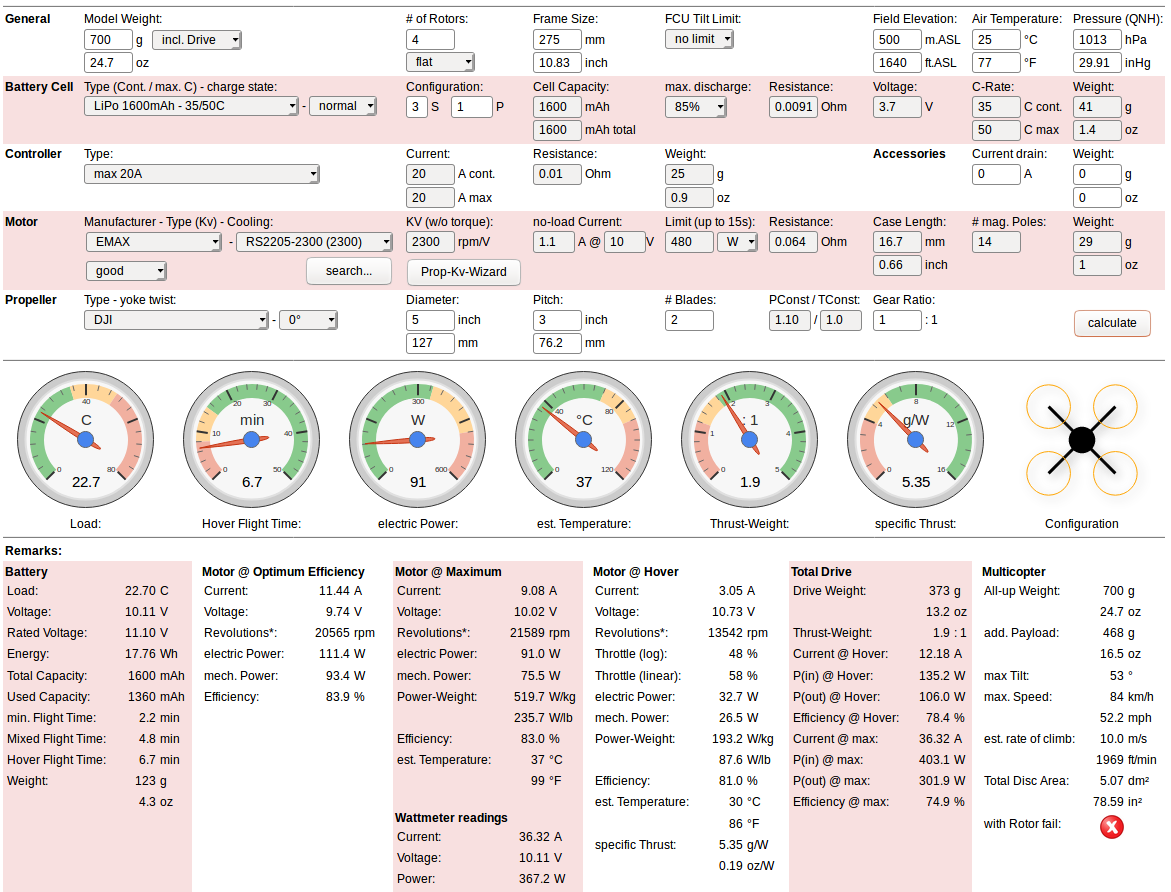
\includegraphics[width=\linewidth]{design/ecalc.png}
    \caption{eCalc copter simulation}
    \label{fig:ecalc}
\end{figure}
